\section{Simulation of Room Acoustics}  \label{sec:simulation}

\begin{figure}[!htp]
\centering
    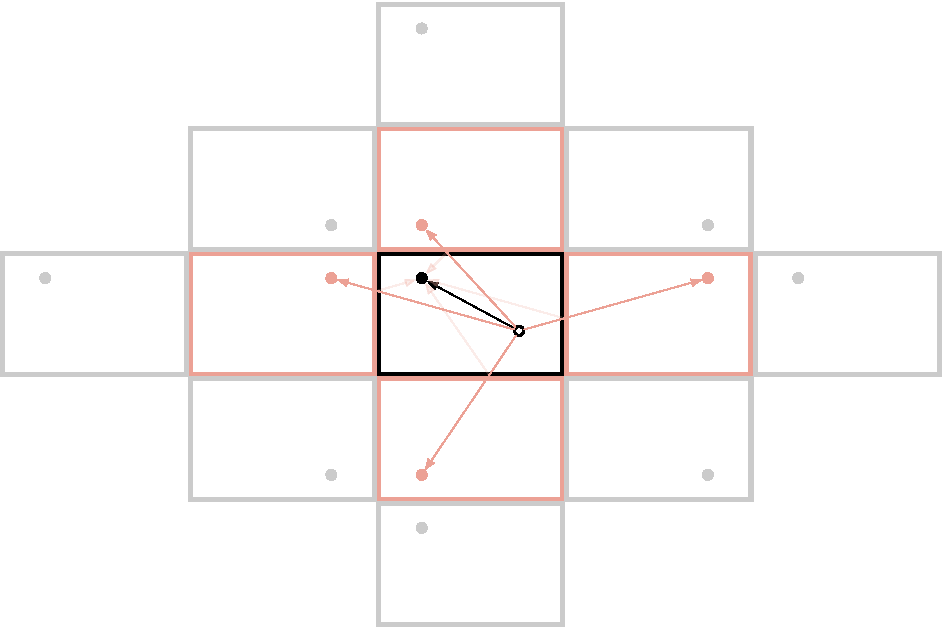
\includegraphics[scale=0.7]{data/figures/image-method2}
    \caption{Second order image expansion for a single source and receiver}
    \label{fig:imageMethod}
\end{figure}

To conduct the experimental part this thesis, simulation as means of data collection has been chosen over real recordings, as simulated acoustic environments are more flexible compared to a laboratory environment. To simulate the experimental setup \alt{in it's different configurations} described in Section \ref{sec:setup}, the image-source method for simulating small-room acoustics is used \cite{Allen1979}. The basic idea of this method is to simulate an arriving signal wave reflected from the walls as a wave arriving directly from a virtual sources, mirrored at the reflecting wall.\alt{direct arrival waves of a mirror image of the room on the reflecting wall.} Based on $T_{60}$, the time it takes the source signal to have decreased by 60dB after the exciting source is switched off, only as many mirror images of the original room are created as can be reached by the signal in that time.

Figure~\ref{fig:imageMethod} shows the second-order image expansion, meaning only received signals of up to two reflections are displayed. The direct propagation path is shown in black, the first order images (including real and virtual propagation paths) are shown in orange and translucent orange respectively, and the second order images (propagation paths omitted) are shown in gray. Whenever the signal crosses a wall into another image (i.e., being reflected), it is attenuated by the wall reflection coefficients $\beta = [\beta_1, \beta_2,\dots,\beta_6]$. There is one coefficient per wall, including the ceiling and the floor, for a total of six coefficients. These wall reflection coefficients can be adjusted to simulate different types of walls, like concrete walls and carpeted walls.

This method allowed for experiments, where a controlled acoustic environment in form of a small, rectangular room is required, that can be easily adjusted. For many experiments\alt{experiments with budget- and time-constraints}, constructing such an environment in a laboratory is prohibitive, which is why the image method has gained widespread popularity since its inception in \citeyear{Allen1979}~\cite{Allen1979} and has been used in a wide range of studies \cite{Champagne1996}.
%TODO: Cite more studies using the image method